% Created by tikzDevice version 0.10.1 on 2016-07-30 22:11:19
% !TEX encoding = UTF-8 Unicode
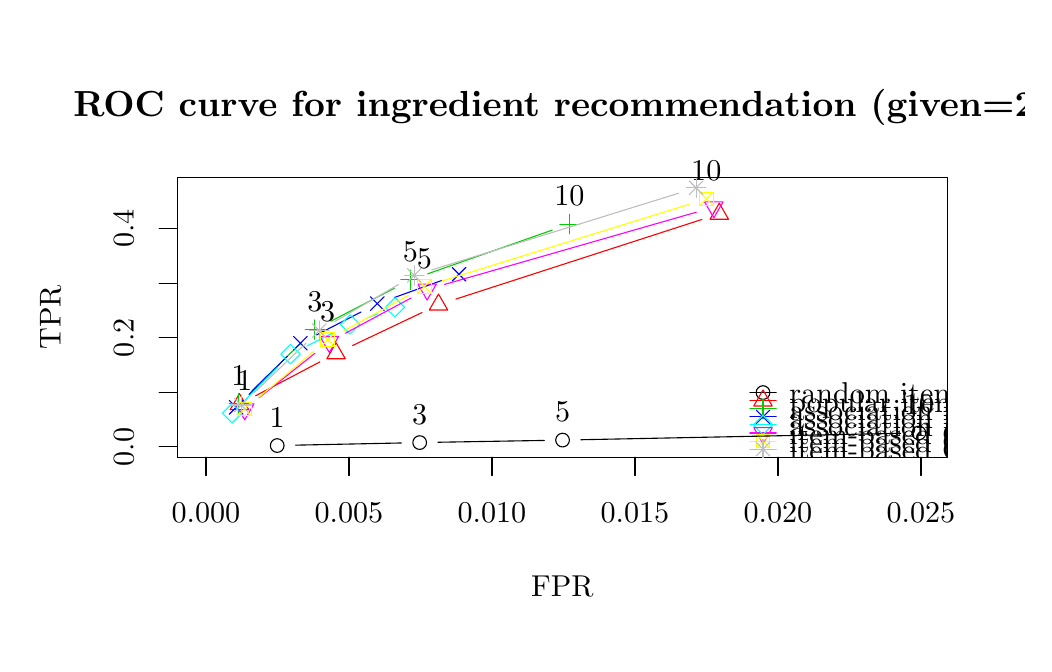
\begin{tikzpicture}[x=1pt,y=1pt]
\definecolor{fillColor}{RGB}{255,255,255}
\path[use as bounding box,fill=fillColor,fill opacity=0.00] (0,0) rectangle (360.07,222.54);
\begin{scope}
\path[clip] (  0.00,  0.00) rectangle (360.07,222.54);
\definecolor{drawColor}{RGB}{0,0,0}

\path[draw=drawColor,line width= 0.4pt,line join=round,line cap=round] ( 64.42, 67.32) -- (322.78, 67.32);

\path[draw=drawColor,line width= 0.4pt,line join=round,line cap=round] ( 64.42, 67.32) -- ( 64.42, 60.72);

\path[draw=drawColor,line width= 0.4pt,line join=round,line cap=round] (116.10, 67.32) -- (116.10, 60.72);

\path[draw=drawColor,line width= 0.4pt,line join=round,line cap=round] (167.77, 67.32) -- (167.77, 60.72);

\path[draw=drawColor,line width= 0.4pt,line join=round,line cap=round] (219.44, 67.32) -- (219.44, 60.72);

\path[draw=drawColor,line width= 0.4pt,line join=round,line cap=round] (271.11, 67.32) -- (271.11, 60.72);

\path[draw=drawColor,line width= 0.4pt,line join=round,line cap=round] (322.78, 67.32) -- (322.78, 60.72);

\node[text=drawColor,anchor=base,inner sep=0pt, outer sep=0pt, scale=  1.09] at ( 64.42, 43.56) {0.000};

\node[text=drawColor,anchor=base,inner sep=0pt, outer sep=0pt, scale=  1.09] at (116.10, 43.56) {0.005};

\node[text=drawColor,anchor=base,inner sep=0pt, outer sep=0pt, scale=  1.09] at (167.77, 43.56) {0.010};

\node[text=drawColor,anchor=base,inner sep=0pt, outer sep=0pt, scale=  1.09] at (219.44, 43.56) {0.015};

\node[text=drawColor,anchor=base,inner sep=0pt, outer sep=0pt, scale=  1.09] at (271.11, 43.56) {0.020};

\node[text=drawColor,anchor=base,inner sep=0pt, outer sep=0pt, scale=  1.09] at (322.78, 43.56) {0.025};

\path[draw=drawColor,line width= 0.4pt,line join=round,line cap=round] ( 54.12, 71.06) -- ( 54.12,149.92);

\path[draw=drawColor,line width= 0.4pt,line join=round,line cap=round] ( 54.12, 71.06) -- ( 47.52, 71.06);

\path[draw=drawColor,line width= 0.4pt,line join=round,line cap=round] ( 54.12, 90.78) -- ( 47.52, 90.78);

\path[draw=drawColor,line width= 0.4pt,line join=round,line cap=round] ( 54.12,110.49) -- ( 47.52,110.49);

\path[draw=drawColor,line width= 0.4pt,line join=round,line cap=round] ( 54.12,130.21) -- ( 47.52,130.21);

\path[draw=drawColor,line width= 0.4pt,line join=round,line cap=round] ( 54.12,149.92) -- ( 47.52,149.92);

\node[text=drawColor,rotate= 90.00,anchor=base,inner sep=0pt, outer sep=0pt, scale=  1.09] at ( 38.28, 71.06) {0.0};

\node[text=drawColor,rotate= 90.00,anchor=base,inner sep=0pt, outer sep=0pt, scale=  1.09] at ( 38.28,110.49) {0.2};

\node[text=drawColor,rotate= 90.00,anchor=base,inner sep=0pt, outer sep=0pt, scale=  1.09] at ( 38.28,149.92) {0.4};

\path[draw=drawColor,line width= 0.4pt,line join=round,line cap=round] ( 54.12, 67.32) --
	(332.35, 67.32) --
	(332.35,168.42) --
	( 54.12,168.42) --
	( 54.12, 67.32);
\end{scope}
\begin{scope}
\path[clip] (  0.00,  0.00) rectangle (360.07,222.54);
\definecolor{drawColor}{RGB}{0,0,0}

\node[text=drawColor,anchor=base,inner sep=0pt, outer sep=0pt, scale=  1.09] at (193.24, 17.16) {FPR};

\node[text=drawColor,rotate= 90.00,anchor=base,inner sep=0pt, outer sep=0pt, scale=  1.09] at ( 11.88,117.87) {TPR};
\end{scope}
\begin{scope}
\path[clip] ( 54.12, 67.32) rectangle (332.35,168.42);
\definecolor{drawColor}{RGB}{0,0,0}

\path[draw=drawColor,line width= 0.4pt,line join=round,line cap=round] (260.95, 90.68) -- (270.48, 90.68);
\definecolor{drawColor}{RGB}{255,0,0}

\path[draw=drawColor,line width= 0.4pt,line join=round,line cap=round] (260.95, 87.76) -- (270.48, 87.76);
\definecolor{drawColor}{RGB}{0,205,0}

\path[draw=drawColor,line width= 0.4pt,line join=round,line cap=round] (260.95, 84.84) -- (270.48, 84.84);
\definecolor{drawColor}{RGB}{0,0,255}

\path[draw=drawColor,line width= 0.4pt,line join=round,line cap=round] (260.95, 81.92) -- (270.48, 81.92);
\definecolor{drawColor}{RGB}{0,255,255}

\path[draw=drawColor,line width= 0.4pt,line join=round,line cap=round] (260.95, 79.00) -- (270.48, 79.00);
\definecolor{drawColor}{RGB}{255,0,255}

\path[draw=drawColor,line width= 0.4pt,line join=round,line cap=round] (260.95, 76.08) -- (270.48, 76.08);
\definecolor{drawColor}{RGB}{255,255,0}

\path[draw=drawColor,line width= 0.4pt,line join=round,line cap=round] (260.95, 73.16) -- (270.48, 73.16);
\definecolor{drawColor}{RGB}{190,190,190}

\path[draw=drawColor,line width= 0.4pt,line join=round,line cap=round] (260.95, 70.24) -- (270.48, 70.24);
\definecolor{drawColor}{RGB}{0,0,0}

\path[draw=drawColor,line width= 0.4pt,line join=round,line cap=round] (265.71, 90.68) circle (  2.47);
\definecolor{drawColor}{RGB}{255,0,0}

\path[draw=drawColor,line width= 0.4pt,line join=round,line cap=round] (265.71, 91.61) --
	(269.05, 85.84) --
	(262.38, 85.84) --
	(265.71, 91.61);
\definecolor{drawColor}{RGB}{0,205,0}

\path[draw=drawColor,line width= 0.4pt,line join=round,line cap=round] (262.21, 84.84) -- (269.21, 84.84);

\path[draw=drawColor,line width= 0.4pt,line join=round,line cap=round] (265.71, 81.34) -- (265.71, 88.34);
\definecolor{drawColor}{RGB}{0,0,255}

\path[draw=drawColor,line width= 0.4pt,line join=round,line cap=round] (263.24, 79.45) -- (268.19, 84.40);

\path[draw=drawColor,line width= 0.4pt,line join=round,line cap=round] (263.24, 84.40) -- (268.19, 79.45);
\definecolor{drawColor}{RGB}{0,255,255}

\path[draw=drawColor,line width= 0.4pt,line join=round,line cap=round] (262.21, 79.00) --
	(265.71, 82.50) --
	(269.21, 79.00) --
	(265.71, 75.50) --
	(262.21, 79.00);
\definecolor{drawColor}{RGB}{255,0,255}

\path[draw=drawColor,line width= 0.4pt,line join=round,line cap=round] (265.71, 72.23) --
	(269.05, 78.01) --
	(262.38, 78.01) --
	(265.71, 72.23);
\definecolor{drawColor}{RGB}{255,255,0}

\path[draw=drawColor,line width= 0.4pt,line join=round,line cap=round] (263.24, 70.69) rectangle (268.19, 75.64);

\path[draw=drawColor,line width= 0.4pt,line join=round,line cap=round] (263.24, 70.69) -- (268.19, 75.64);

\path[draw=drawColor,line width= 0.4pt,line join=round,line cap=round] (263.24, 75.64) -- (268.19, 70.69);
\definecolor{drawColor}{RGB}{190,190,190}

\path[draw=drawColor,line width= 0.4pt,line join=round,line cap=round] (263.24, 67.77) -- (268.19, 72.72);

\path[draw=drawColor,line width= 0.4pt,line join=round,line cap=round] (263.24, 72.72) -- (268.19, 67.77);

\path[draw=drawColor,line width= 0.4pt,line join=round,line cap=round] (262.21, 70.24) -- (269.21, 70.24);

\path[draw=drawColor,line width= 0.4pt,line join=round,line cap=round] (265.71, 66.74) -- (265.71, 73.74);
\definecolor{drawColor}{RGB}{0,0,0}

\node[text=drawColor,anchor=base west,inner sep=0pt, outer sep=0pt, scale=  1.09] at (275.24, 86.57) {random items};

\node[text=drawColor,anchor=base west,inner sep=0pt, outer sep=0pt, scale=  1.09] at (275.24, 83.65) {popular items};

\node[text=drawColor,anchor=base west,inner sep=0pt, outer sep=0pt, scale=  1.09] at (275.24, 80.73) {association rules (0.01)};

\node[text=drawColor,anchor=base west,inner sep=0pt, outer sep=0pt, scale=  1.09] at (275.24, 77.81) {association rules (0.05)};

\node[text=drawColor,anchor=base west,inner sep=0pt, outer sep=0pt, scale=  1.09] at (275.24, 74.89) {association rules (0.1)};

\node[text=drawColor,anchor=base west,inner sep=0pt, outer sep=0pt, scale=  1.09] at (275.24, 71.97) {item-based CF (k=20)};

\node[text=drawColor,anchor=base west,inner sep=0pt, outer sep=0pt, scale=  1.09] at (275.24, 69.05) {item-based CF (k=40)};

\node[text=drawColor,anchor=base west,inner sep=0pt, outer sep=0pt, scale=  1.09] at (275.24, 66.13) {item-based CF (k=200)};

\path[draw=drawColor,line width= 0.4pt,line join=round,line cap=round] ( 96.77, 71.68) -- (135.05, 72.47);

\path[draw=drawColor,line width= 0.4pt,line join=round,line cap=round] (148.25, 72.73) -- (186.68, 73.39);

\path[draw=drawColor,line width= 0.4pt,line join=round,line cap=round] (199.88, 73.64) -- (315.45, 75.96);

\path[draw=drawColor,line width= 0.4pt,line join=round,line cap=round] ( 90.17, 71.54) circle (  2.47);

\path[draw=drawColor,line width= 0.4pt,line join=round,line cap=round] (141.65, 72.61) circle (  2.47);

\path[draw=drawColor,line width= 0.4pt,line join=round,line cap=round] (193.28, 73.51) circle (  2.47);

\path[draw=drawColor,line width= 0.4pt,line join=round,line cap=round] (322.05, 76.09) circle (  2.47);
\end{scope}
\begin{scope}
\path[clip] (  0.00,  0.00) rectangle (360.07,222.54);
\definecolor{drawColor}{RGB}{0,0,0}

\node[text=drawColor,anchor=base,inner sep=0pt, outer sep=0pt, scale=  1.09] at ( 90.17, 78.14) {1};

\node[text=drawColor,anchor=base,inner sep=0pt, outer sep=0pt, scale=  1.09] at (141.65, 79.21) {3};

\node[text=drawColor,anchor=base,inner sep=0pt, outer sep=0pt, scale=  1.09] at (193.28, 80.11) {5};

\node[text=drawColor,anchor=base,inner sep=0pt, outer sep=0pt, scale=  1.09] at (322.05, 82.69) {10};
\end{scope}
\begin{scope}
\path[clip] ( 54.12, 67.32) rectangle (332.35,168.42);
\definecolor{drawColor}{RGB}{255,0,0}

\path[draw=drawColor,line width= 0.4pt,line join=round,line cap=round] ( 82.36, 89.53) -- (105.60,101.77);

\path[draw=drawColor,line width= 0.4pt,line join=round,line cap=round] (117.40,107.68) -- (142.50,119.60);

\path[draw=drawColor,line width= 0.4pt,line join=round,line cap=round] (154.74,124.47) -- (243.62,153.23);

\path[draw=drawColor,line width= 0.4pt,line join=round,line cap=round] ( 76.52, 90.31) --
	( 79.86, 84.53) --
	( 73.19, 84.53) --
	( 76.52, 90.31);

\path[draw=drawColor,line width= 0.4pt,line join=round,line cap=round] (111.44,108.69) --
	(114.77,102.92) --
	(108.11,102.92) --
	(111.44,108.69);

\path[draw=drawColor,line width= 0.4pt,line join=round,line cap=round] (148.46,126.28) --
	(151.79,120.51) --
	(145.12,120.51) --
	(148.46,126.28);

\path[draw=drawColor,line width= 0.4pt,line join=round,line cap=round] (249.90,159.11) --
	(253.24,153.33) --
	(246.57,153.33) --
	(249.90,159.11);
\definecolor{drawColor}{RGB}{0,205,0}

\path[draw=drawColor,line width= 0.4pt,line join=round,line cap=round] ( 81.05, 91.39) -- ( 99.05,108.86);

\path[draw=drawColor,line width= 0.4pt,line join=round,line cap=round] (109.64,116.50) -- (132.47,128.37);

\path[draw=drawColor,line width= 0.4pt,line join=round,line cap=round] (144.55,133.60) -- (189.55,149.38);

\path[draw=drawColor,line width= 0.4pt,line join=round,line cap=round] ( 72.82, 86.80) -- ( 79.82, 86.80);

\path[draw=drawColor,line width= 0.4pt,line join=round,line cap=round] ( 76.32, 83.30) -- ( 76.32, 90.30);

\path[draw=drawColor,line width= 0.4pt,line join=round,line cap=round] (100.29,113.46) -- (107.29,113.46);

\path[draw=drawColor,line width= 0.4pt,line join=round,line cap=round] (103.79,109.96) -- (103.79,116.96);

\path[draw=drawColor,line width= 0.4pt,line join=round,line cap=round] (134.82,131.41) -- (141.82,131.41);

\path[draw=drawColor,line width= 0.4pt,line join=round,line cap=round] (138.32,127.91) -- (138.32,134.91);

\path[draw=drawColor,line width= 0.4pt,line join=round,line cap=round] (192.28,151.56) -- (199.28,151.56);

\path[draw=drawColor,line width= 0.4pt,line join=round,line cap=round] (195.78,148.06) -- (195.78,155.06);
\end{scope}
\begin{scope}
\path[clip] (  0.00,  0.00) rectangle (360.07,222.54);
\definecolor{drawColor}{RGB}{0,0,0}

\node[text=drawColor,anchor=base,inner sep=0pt, outer sep=0pt, scale=  1.09] at ( 76.32, 93.40) {1};

\node[text=drawColor,anchor=base,inner sep=0pt, outer sep=0pt, scale=  1.09] at (103.79,120.06) {3};

\node[text=drawColor,anchor=base,inner sep=0pt, outer sep=0pt, scale=  1.09] at (138.32,138.01) {5};

\node[text=drawColor,anchor=base,inner sep=0pt, outer sep=0pt, scale=  1.09] at (195.78,158.16) {10};
\end{scope}
\begin{scope}
\path[clip] ( 54.12, 67.32) rectangle (332.35,168.42);
\definecolor{drawColor}{RGB}{0,0,255}

\path[draw=drawColor,line width= 0.4pt,line join=round,line cap=round] ( 80.00, 90.01) -- ( 93.85,103.84);

\path[draw=drawColor,line width= 0.4pt,line join=round,line cap=round] (104.39,111.53) -- (120.45,119.79);

\path[draw=drawColor,line width= 0.4pt,line join=round,line cap=round] (132.53,125.04) -- (149.66,131.20);

\path[draw=drawColor,line width= 0.4pt,line join=round,line cap=round] ( 72.86, 82.87) -- ( 77.81, 87.82);

\path[draw=drawColor,line width= 0.4pt,line join=round,line cap=round] ( 72.86, 87.82) -- ( 77.81, 82.87);

\path[draw=drawColor,line width= 0.4pt,line join=round,line cap=round] ( 96.05,106.03) -- (101.00,110.98);

\path[draw=drawColor,line width= 0.4pt,line join=round,line cap=round] ( 96.05,110.98) -- (101.00,106.03);

\path[draw=drawColor,line width= 0.4pt,line join=round,line cap=round] (123.85,120.33) -- (128.80,125.28);

\path[draw=drawColor,line width= 0.4pt,line join=round,line cap=round] (123.85,125.28) -- (128.80,120.33);

\path[draw=drawColor,line width= 0.4pt,line join=round,line cap=round] (153.39,130.96) -- (158.34,135.91);

\path[draw=drawColor,line width= 0.4pt,line join=round,line cap=round] (153.39,135.91) -- (158.34,130.96);
\definecolor{drawColor}{RGB}{0,255,255}

\path[draw=drawColor,line width= 0.4pt,line join=round,line cap=round] ( 78.49, 87.89) -- ( 90.34, 99.88);

\path[draw=drawColor,line width= 0.4pt,line join=round,line cap=round] (100.88,107.52) -- (110.60,112.37);

\path[draw=drawColor,line width= 0.4pt,line join=round,line cap=round] (122.67,117.66) -- (126.53,119.13);

\path[draw=drawColor,line width= 0.4pt,line join=round,line cap=round] ( 70.35, 83.20) --
	( 73.85, 86.70) --
	( 77.35, 83.20) --
	( 73.85, 79.70) --
	( 70.35, 83.20);

\path[draw=drawColor,line width= 0.4pt,line join=round,line cap=round] ( 91.48,104.58) --
	( 94.98,108.08) --
	( 98.48,104.58) --
	( 94.98,101.07) --
	( 91.48,104.58);

\path[draw=drawColor,line width= 0.4pt,line join=round,line cap=round] (113.00,115.31) --
	(116.50,118.81) --
	(120.00,115.31) --
	(116.50,111.81) --
	(113.00,115.31);

\path[draw=drawColor,line width= 0.4pt,line join=round,line cap=round] (129.20,121.48) --
	(132.70,124.98) --
	(136.20,121.48) --
	(132.70,117.98) --
	(129.20,121.48);
\definecolor{drawColor}{RGB}{255,0,255}

\path[draw=drawColor,line width= 0.4pt,line join=round,line cap=round] ( 83.59, 88.80) -- (103.83,104.90);

\path[draw=drawColor,line width= 0.4pt,line join=round,line cap=round] (114.81,112.13) -- (138.52,124.84);

\path[draw=drawColor,line width= 0.4pt,line join=round,line cap=round] (150.68,129.77) -- (241.59,155.85);

\path[draw=drawColor,line width= 0.4pt,line join=round,line cap=round] ( 78.43, 80.84) --
	( 81.76, 86.61) --
	( 75.09, 86.61) --
	( 78.43, 80.84);

\path[draw=drawColor,line width= 0.4pt,line join=round,line cap=round] (108.99,105.16) --
	(112.33,110.93) --
	(105.66,110.93) --
	(108.99,105.16);

\path[draw=drawColor,line width= 0.4pt,line join=round,line cap=round] (144.33,124.11) --
	(147.67,129.88) --
	(141.00,129.88) --
	(144.33,124.11);

\path[draw=drawColor,line width= 0.4pt,line join=round,line cap=round] (247.94,153.82) --
	(251.27,159.59) --
	(244.60,159.59) --
	(247.94,153.82);
\definecolor{drawColor}{RGB}{255,255,0}

\path[draw=drawColor,line width= 0.4pt,line join=round,line cap=round] ( 83.50, 88.96) -- (103.35,105.53);

\path[draw=drawColor,line width= 0.4pt,line join=round,line cap=round] (114.20,112.94) -- (137.61,125.85);

\path[draw=drawColor,line width= 0.4pt,line join=round,line cap=round] (149.70,131.00) -- (238.93,158.69);

\path[draw=drawColor,line width= 0.4pt,line join=round,line cap=round] ( 75.95, 82.26) rectangle ( 80.90, 87.21);

\path[draw=drawColor,line width= 0.4pt,line join=round,line cap=round] ( 75.95, 82.26) -- ( 80.90, 87.21);

\path[draw=drawColor,line width= 0.4pt,line join=round,line cap=round] ( 75.95, 87.21) -- ( 80.90, 82.26);

\path[draw=drawColor,line width= 0.4pt,line join=round,line cap=round] (105.94,107.28) rectangle (110.89,112.23);

\path[draw=drawColor,line width= 0.4pt,line join=round,line cap=round] (105.94,107.28) -- (110.89,112.23);

\path[draw=drawColor,line width= 0.4pt,line join=round,line cap=round] (105.94,112.23) -- (110.89,107.28);

\path[draw=drawColor,line width= 0.4pt,line join=round,line cap=round] (140.92,126.57) rectangle (145.87,131.52);

\path[draw=drawColor,line width= 0.4pt,line join=round,line cap=round] (140.92,126.57) -- (145.87,131.52);

\path[draw=drawColor,line width= 0.4pt,line join=round,line cap=round] (140.92,131.52) -- (145.87,126.57);

\path[draw=drawColor,line width= 0.4pt,line join=round,line cap=round] (242.76,158.17) rectangle (247.71,163.12);

\path[draw=drawColor,line width= 0.4pt,line join=round,line cap=round] (242.76,158.17) -- (247.71,163.12);

\path[draw=drawColor,line width= 0.4pt,line join=round,line cap=round] (242.76,163.12) -- (247.71,158.17);
\end{scope}
\begin{scope}
\path[clip] (  0.00,  0.00) rectangle (360.07,222.54);
\definecolor{drawColor}{RGB}{0,0,0}

\node[text=drawColor,anchor=base,inner sep=0pt, outer sep=0pt, scale=  1.09] at ( 78.43, 91.34) {1};

\node[text=drawColor,anchor=base,inner sep=0pt, outer sep=0pt, scale=  1.09] at (108.42,116.35) {3};

\node[text=drawColor,anchor=base,inner sep=0pt, outer sep=0pt, scale=  1.09] at (143.39,135.64) {5};

\node[text=drawColor,anchor=base,inner sep=0pt, outer sep=0pt, scale=  1.09] at (245.23,167.24) {10};
\end{scope}
\begin{scope}
\path[clip] ( 54.12, 67.32) rectangle (332.35,168.42);
\definecolor{drawColor}{RGB}{190,190,190}

\path[draw=drawColor,line width= 0.4pt,line join=round,line cap=round] ( 81.95, 90.74) -- (100.58,108.52);

\path[draw=drawColor,line width= 0.4pt,line join=round,line cap=round] (111.06,116.39) -- (133.97,129.72);

\path[draw=drawColor,line width= 0.4pt,line join=round,line cap=round] (145.98,134.99) -- (235.23,162.72);

\path[draw=drawColor,line width= 0.4pt,line join=round,line cap=round] ( 74.70, 83.70) -- ( 79.65, 88.65);

\path[draw=drawColor,line width= 0.4pt,line join=round,line cap=round] ( 74.70, 88.65) -- ( 79.65, 83.70);

\path[draw=drawColor,line width= 0.4pt,line join=round,line cap=round] ( 73.68, 86.18) -- ( 80.68, 86.18);

\path[draw=drawColor,line width= 0.4pt,line join=round,line cap=round] ( 77.18, 82.68) -- ( 77.18, 89.68);

\path[draw=drawColor,line width= 0.4pt,line join=round,line cap=round] (102.87,110.60) -- (107.82,115.55);

\path[draw=drawColor,line width= 0.4pt,line join=round,line cap=round] (102.87,115.55) -- (107.82,110.60);

\path[draw=drawColor,line width= 0.4pt,line join=round,line cap=round] (101.85,113.08) -- (108.85,113.08);

\path[draw=drawColor,line width= 0.4pt,line join=round,line cap=round] (105.35,109.58) -- (105.35,116.58);

\path[draw=drawColor,line width= 0.4pt,line join=round,line cap=round] (137.21,130.56) -- (142.16,135.51);

\path[draw=drawColor,line width= 0.4pt,line join=round,line cap=round] (137.21,135.51) -- (142.16,130.56);

\path[draw=drawColor,line width= 0.4pt,line join=round,line cap=round] (136.18,133.04) -- (143.18,133.04);

\path[draw=drawColor,line width= 0.4pt,line join=round,line cap=round] (139.68,129.53) -- (139.68,136.54);

\path[draw=drawColor,line width= 0.4pt,line join=round,line cap=round] (239.05,162.20) -- (244.00,167.15);

\path[draw=drawColor,line width= 0.4pt,line join=round,line cap=round] (239.05,167.15) -- (244.00,162.20);

\path[draw=drawColor,line width= 0.4pt,line join=round,line cap=round] (238.03,164.68) -- (245.03,164.68);

\path[draw=drawColor,line width= 0.4pt,line join=round,line cap=round] (241.53,161.18) -- (241.53,168.18);
\end{scope}
\begin{scope}
\path[clip] (  0.00,  0.00) rectangle (360.07,222.54);
\definecolor{drawColor}{RGB}{0,0,0}

\node[text=drawColor,anchor=base,inner sep=0pt, outer sep=0pt, scale=  1.31] at (193.24,190.53) {\bfseries ROC curve for ingredient recommendation (given=2)};
\end{scope}
\end{tikzpicture}
